% GNUPLOT: LaTeX picture with Postscript
\begingroup
  \makeatletter
  \providecommand\color[2][]{%
    \GenericError{(gnuplot) \space\space\space\@spaces}{%
      Package color not loaded in conjunction with
      terminal option `colourtext'%
    }{See the gnuplot documentation for explanation.%
    }{Either use 'blacktext' in gnuplot or load the package
      color.sty in LaTeX.}%
    \renewcommand\color[2][]{}%
  }%
  \providecommand\includegraphics[2][]{%
    \GenericError{(gnuplot) \space\space\space\@spaces}{%
      Package graphicx or graphics not loaded%
    }{See the gnuplot documentation for explanation.%
    }{The gnuplot epslatex terminal needs graphicx.sty or graphics.sty.}%
    \renewcommand\includegraphics[2][]{}%
  }%
  \providecommand\rotatebox[2]{#2}%
  \@ifundefined{ifGPcolor}{%
    \newif\ifGPcolor
    \GPcolortrue
  }{}%
  \@ifundefined{ifGPblacktext}{%
    \newif\ifGPblacktext
    \GPblacktextfalse
  }{}%
  % define a \g@addto@macro without @ in the name:
  \let\gplgaddtomacro\g@addto@macro
  % define empty templates for all commands taking text:
  \gdef\gplbacktext{}%
  \gdef\gplfronttext{}%
  \makeatother
  \ifGPblacktext
    % no textcolor at all
    \def\colorrgb#1{}%
    \def\colorgray#1{}%
  \else
    % gray or color?
    \ifGPcolor
      \def\colorrgb#1{\color[rgb]{#1}}%
      \def\colorgray#1{\color[gray]{#1}}%
      \expandafter\def\csname LTw\endcsname{\color{white}}%
      \expandafter\def\csname LTb\endcsname{\color{black}}%
      \expandafter\def\csname LTa\endcsname{\color{black}}%
      \expandafter\def\csname LT0\endcsname{\color[rgb]{1,0,0}}%
      \expandafter\def\csname LT1\endcsname{\color[rgb]{0,1,0}}%
      \expandafter\def\csname LT2\endcsname{\color[rgb]{0,0,1}}%
      \expandafter\def\csname LT3\endcsname{\color[rgb]{1,0,1}}%
      \expandafter\def\csname LT4\endcsname{\color[rgb]{0,1,1}}%
      \expandafter\def\csname LT5\endcsname{\color[rgb]{1,1,0}}%
      \expandafter\def\csname LT6\endcsname{\color[rgb]{0,0,0}}%
      \expandafter\def\csname LT7\endcsname{\color[rgb]{1,0.3,0}}%
      \expandafter\def\csname LT8\endcsname{\color[rgb]{0.5,0.5,0.5}}%
    \else
      % gray
      \def\colorrgb#1{\color{black}}%
      \def\colorgray#1{\color[gray]{#1}}%
      \expandafter\def\csname LTw\endcsname{\color{white}}%
      \expandafter\def\csname LTb\endcsname{\color{black}}%
      \expandafter\def\csname LTa\endcsname{\color{black}}%
      \expandafter\def\csname LT0\endcsname{\color{black}}%
      \expandafter\def\csname LT1\endcsname{\color{black}}%
      \expandafter\def\csname LT2\endcsname{\color{black}}%
      \expandafter\def\csname LT3\endcsname{\color{black}}%
      \expandafter\def\csname LT4\endcsname{\color{black}}%
      \expandafter\def\csname LT5\endcsname{\color{black}}%
      \expandafter\def\csname LT6\endcsname{\color{black}}%
      \expandafter\def\csname LT7\endcsname{\color{black}}%
      \expandafter\def\csname LT8\endcsname{\color{black}}%
    \fi
  \fi
  \setlength{\unitlength}{0.0500bp}%
  \begin{picture}(4818.00,4250.00)%
    \gplgaddtomacro\gplbacktext{%
      \csname LTb\endcsname%
      \put(550,704){\makebox(0,0)[r]{\strut{}$0$}}%
      \put(550,1025){\makebox(0,0)[r]{\strut{}$1$}}%
      \put(550,1345){\makebox(0,0)[r]{\strut{}$2$}}%
      \put(550,1666){\makebox(0,0)[r]{\strut{}$3$}}%
      \put(550,1986){\makebox(0,0)[r]{\strut{}$4$}}%
      \put(550,2307){\makebox(0,0)[r]{\strut{}$5$}}%
      \put(550,2627){\makebox(0,0)[r]{\strut{}$6$}}%
      \put(550,2948){\makebox(0,0)[r]{\strut{}$7$}}%
      \put(550,3268){\makebox(0,0)[r]{\strut{}$8$}}%
      \put(550,3589){\makebox(0,0)[r]{\strut{}$9$}}%
      \put(682,484){\makebox(0,0){\strut{}$0$}}%
      \put(1181,484){\makebox(0,0){\strut{}$0.2$}}%
      \put(1679,484){\makebox(0,0){\strut{}$0.4$}}%
      \put(2178,484){\makebox(0,0){\strut{}$0.6$}}%
      \put(2676,484){\makebox(0,0){\strut{}$0.8$}}%
      \put(3175,484){\makebox(0,0){\strut{}$1$}}%
      \put(3673,484){\makebox(0,0){\strut{}$1.2$}}%
      \put(4172,484){\makebox(0,0){\strut{}$1.4$}}%
      \put(176,2146){\rotatebox{-270}{\makebox(0,0){\strut{}$y$}}}%
      \put(2551,154){\makebox(0,0){\strut{}$x$}}%
      \put(2551,3919){\makebox(0,0){\strut{}Hauptisoklinen des Brusselators mit $a, b = \mathrm{const.}$, Trapping-Region (Poincar\'e-Bendixson)}}%
      \put(3206,1697){\makebox(0,0)[l]{\strut{} }}%
      \put(2925,1906){\makebox(0,0)[l]{\strut{}fixed point}}%
    }%
    \gplgaddtomacro\gplfronttext{%
      \csname LTb\endcsname%
      \put(3434,3416){\makebox(0,0)[r]{\strut{}$\dot{x} = 0$}}%
      \csname LTb\endcsname%
      \put(3434,3196){\makebox(0,0)[r]{\strut{}$\dot{y} = 0$}}%
    }%
    \gplbacktext
    \put(0,0){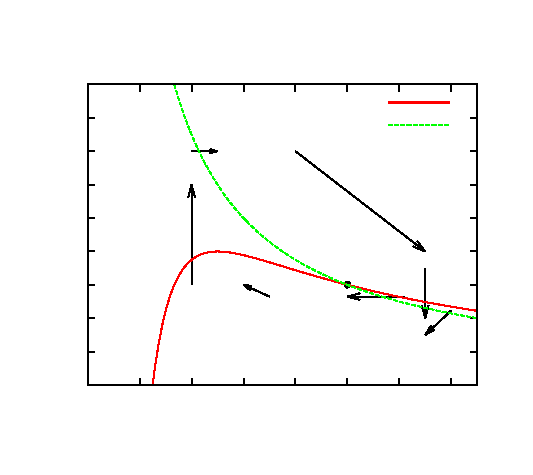
\includegraphics{trappingreg}}%
    \gplfronttext
  \end{picture}%
\endgroup
